\documentclass[11pt]{article}

% ------------------------------------------------------------------
% Exposição à IA em um Mercado de Trabalho Informal
% Artigo misto teoria-empírica — esqueleto de trabalho
% Compilar: latexmk -pdf main.tex  (ou pdflatex + bibtex + pdflatex x2)
% ------------------------------------------------------------------

\usepackage[T1]{fontenc}
\usepackage[utf8]{inputenc}
\usepackage[brazilian]{babel}
\usepackage[margin=1in]{geometry}
\usepackage{amsmath,amssymb,amsthm}
\usepackage{graphicx}
\usepackage{booktabs}
\usepackage{caption}
\usepackage{microtype}
\usepackage[round,authoryear]{natbib}
\usepackage[colorlinks=true,linkcolor=blue,citecolor=blue,urlcolor=blue]{hyperref}

\captionsetup{font=small,labelfont=bf}
\newtheorem{proposicao}{Proposição}
\newtheorem{corolario}{Corolário}

% Nota de rodapé de título (agradecimentos, dados, contato)
\title{Exposição à Inteligência Artificial em um Mercado de Trabalho Informal: Teoria e Evidências para o Brasil\thanks{Bacharel em Economia pela Universidade de Coimbra. Os microdados da PNAD Contínua são públicos (IBGE); o código de replicação e o painel de dados estão disponíveis no repositório do projeto.}}
\author{Marcelo Moura Freire}
\date{\today}

\begin{document}

\maketitle

\begin{abstract}
\noindent
Quanto do mercado de trabalho brasileiro está efetivamente sujeito à inteligência artificial --- e quem são os expostos? Este artigo desenvolve um modelo de designação de tarefas com adoção corporativa e individual de IA sob informalidade, e testa suas previsões nos microdados da PNAD Contínua, combinados ao índice de \citet{eloundou2024gpts} por um cruzamento ocupacional determinístico. A exposição concentra-se no núcleo formal e escolarizado: 35\% da força de trabalho (35{,}7 milhões de pessoas) atua em ocupações de exposição quase nula ($\theta \le 2$). Em modelos no nível do indivíduo com controles mincerianos completos (idade, gênero e raça), cada ano adicional de estudo associa-se a 0{,}23 ponto a mais de exposição à IA (erro-padrão 0{,}03 agrupado em 122 ocupações; $N = 227.629$). A associação entre exposição e formalidade é robusta, e o gradiente é mais íngreme nas 27 Unidades da Federação com setor formal mais profundo. No Brasil, a informalidade funciona como o principal amortecedor da exposição à IA.
\end{abstract}


\section{Introdução}
\label{sec:intro}

Trinta e cinco milhões de brasileiros --- 35\% da força de trabalho ocupada --- atuam em ocupações com exposição quase nula à inteligência artificial ($\theta \le 2$ em uma escala de 0 a 10). Não é a sofisticação das tarefas que as isola, mas o caráter predominantemente manual, presencial e informal de suas atividades. O trabalho doméstico (6{,}7 milhões de postos) e a construção civil estrutural (3{,}2 milhões) somam mais empregos do que todas as ocupações de tecnologia, finanças e administração somadas; sua exposição ao índice de \citet{eloundou2024gpts} é de 0{,}1 e 0{,}9, respectivamente, contra 7{,}5 dos desenvolvedores de software e 8{,}6 dos operadores de máquinas de escritório.

Esse quadro qualifica a narrativa dominante sobre IA e mercado de trabalho. Nos Estados Unidos, \citet{eloundou2024gpts} estimam que cerca de 80\% da força de trabalho tem ao menos 10\% de suas tarefas afetadas por grandes modelos de linguagem. No Brasil, a mesma métrica revela um padrão assimétrico: a exposição é \emph{positivamente} associada à escolaridade e à renda, concentrando-se no emprego formal. O mercado de trabalho brasileiro conta com um amortecedor ausente nas economias avançadas --- a informalidade ---, e esse amortecedor situa-se exatamente na base do espectro de exposição.

Este artigo investiga quem, no mercado de trabalho brasileiro, está exposto à IA e por meio de quais mecanismos econômicos. Desenvolvo um modelo de designação de tarefas com setor informal em que a IA individual está universalmente disponível, mas a IA corporativa exige capital organizacional restrito à formalidade. Testo as previsões do modelo com os microdados trimestrais da PNAD Contínua (2026Q1, com mais de 227 mil trabalhadores analisados individualmente), combinados ao mapeamento determinístico entre a COD brasileira e a classificação O*NET-SOC.

Três resultados empíricos emergem. Primeiro, a exposição ordena-se fortemente com a escolaridade: com controles mincerianos completos (idade, idade ao quadrado, gênero e raça) e erros-padrão agrupados por ocupação (122 grupos), cada ano adicional de estudo associa-se a 0{,}23 ponto a mais de exposição à IA (erro-padrão 0{,}03; $p < 0{,}001$; $N = 227.629$). Segundo, a associação entre exposição e formalidade é marcante: na relação incondicional, cada ponto de exposição associa-se a $-6{,}23$ p.p. de informalidade ($p < 0{,}001$). Condicional à escolaridade individual, o coeficiente da exposição atenua-se em $37{,}2\%$ para $-3{,}91$ p.p. (erro-padrão 0{,}96), enquanto cada ano de escolaridade associa-se a $-2{,}61$ p.p. de informalidade ($p < 0{,}001$), evidenciando a mediação parcial pelo capital humano e a persistência de um canal tecnológico direto. Terceiro, o gradiente educacional é mais acentuado nas Unidades da Federação com maior maturidade do setor formal: a interação entre escolaridade e a formalidade da UF (calculada via \emph{leave-one-out}) é de 0{,}28 (erro-padrão 0{,}06; $p < 0{,}001$).

A interpretação desses padrões é de \emph{sorting} ocupacional de equilíbrio, não de impacto causal ou deslocamento imediato de trabalhadores. O modelo formaliza essa distinção: trabalhadores mais escolarizados possuem vantagem comparativa em tarefas cognitivas e abstratas complementares à IA, auto-selecionando-se nas ocupações mais expostas do setor formal, onde o retorno ao capital organizacional corporativo compensa os custos de conformidade tributária e regulatória.

O artigo conecta três literaturas. A primeira mensura a exposição das ocupações a novas tecnologias \citep{frey2017future,acemoglu2022tasks,eloundou2024gpts}, desenvolvida primordialmente para economias formais; dentro dela, a automação desloca e reinstata tarefas \citep{acemoglu2019automation}, e o emprego persiste porque máquinas complementam --- e não apenas substituem --- trabalho \citep{autor2015why}. A segunda analisa a escolha entre formalidade e informalidade em economias em desenvolvimento \citep{ulyssea2018firms}. A terceira modela a alocação de trabalhadores a tarefas \citep{acemoglu2011skills,autordorn2013growth}.

A contribuição do trabalho é tripla: (i) apresenta a primeira mensuração em nível de microdados da exposição à IA para o Brasil com controles demográficos completos e inferência robusta; (ii) formaliza a barreira do capital organizacional corporativo como mediador da exposição tecnológica sob informalidade; e (iii) qualifica o debate de políticas públicas, indicando que as políticas de adaptação e capacitação em IA devem focar no estrato médio formal escolarizado, hoje o mais exposto aos choques tecnológicos.

A Seção~\ref{sec:modelo} apresenta o modelo teórico; a Seção~\ref{sec:dados} descreve os microdados e o cruzamento ocupacional; a Seção~\ref{sec:estrategia} detalha a estratégia empírica; a Seção~\ref{sec:resultados} discute as estimativas e testes de robustez; e a Seção~\ref{sec:conclusao} conclui.


% ==================================================================
% MODELO — Princípios: modelo mais simples que gera o insight;
% ambiente em texto corrido ANTES da matemática; suposições numeradas
% com conteúdo econômico explícito; proposições com intuição ANTES da
% demonstração; provas no apêndice. Cada proposição gera uma previsão
% testável mapeada a uma regressão da Seção 4.
% ==================================================================
\section{Modelo}
\label{sec:modelo}

\subsection{Ambiente}

Apresento um modelo estático de designação ocupacional em equilíbrio parcial com dois setores contratuais --- formal ($F$) e informal ($I$) --- e um contínuo de trabalhadores com escolaridade heterogênea $e \in [e_{\min}, e_{\max}]$, distribuídos segundo uma função de densidade contínua $f(e)$. A economia dispõe de $J$ ocupações distintas, indexadas por $j \in \{1, \dots, J\}$. Cada ocupação é caracterizada por um vetor fixo de tarefas com índice de exposição tecnológica à inteligência artificial $\theta_j \in [0, 10]$, determinado exogenamente pelas características intrínsecas das rotinas informacionais \citep{eloundou2024gpts}. 

Os trabalhadores escolhem simultaneamente a ocupação $j$ e o arranjo contratual $s \in \{F, I\}$ para maximizar sua remuneração líquida, tomando os parâmetros tecnológicos e os custos regulatórios como dados. Firmas do setor formal incorrem em um custo fixo de conformidade tributária e institucional $c > 0$ por trabalhador \citep{ulyssea2018firms}, mas fornecem infraestrutura corporativa, capital de dados proprietários e governança que potencializam os ganhos de produtividade proporcionados pela IA. No setor informal, os trabalhadores acessam livremente ferramentas individuais de IA (como assistentes generativos em dispositivos pessoais), mas não dispõem do capital complementar organizacional necessário para converter a tecnologia em ganhos corporativos de escala.

Em termos econômicos, a IA opera como uma tecnologia de tarefas informacionais. Embora aplicativos generativos sejam universalmente acessíveis a qualquer indivíduo com conexão digital, a escala de integração corporativa --- integração a fluxos de trabalho estruturados, segurança da informação e governança de dados --- requer formalização. Assim, a informalidade amortece a exposição à automação não por erguer uma barreira física de acesso à ferramenta, mas por limitar a rentabilidade econômica da integração tecnológica corporativa.

\subsection{Primitivos de produção e salários}

Um trabalhador com escolaridade $e$ alocado à ocupação $j$ sob o arranjo contratual $s \in \{F, I\}$ gera produto
\begin{equation}
    y_{j s}(e) = g(e) \, \big(1 + \kappa_s \, \theta_j\big),
    \label{eq:produto}
\end{equation}
onde $g(e)$ (com $g' > 0$ e $g'' \le 0$) representa o componente básico de capital humano, e $\kappa_s > 0$ parametriza a eficácia da IA sob o arranjo $s$. Defino a estrutura de retorno tecnológico por:
\begin{equation}
    \kappa_s = \kappa_{\text{ind}} + \Delta\kappa \, \mathbb{1}[s = F], \quad \text{com } \Delta\kappa \equiv \kappa_{\text{org}} - \kappa_{\text{ind}} > 0,
\end{equation}
em que $\kappa_{\text{ind}} \ge 0$ captura o ganho da IA individual autônoma (disponível universalmente) e $\Delta\kappa > 0$ reflete o \emph{prêmio de capital organizacional} restrito às empresas do setor formal.

Sob concorrência perfeita no mercado de trabalho e preços de tarefas normalizados a um, a remuneração de equilíbrio iguala a produtividade líquida do custo de conformidade regulatória:
\begin{equation}
    w_{jF}(e) = y_{jF}(e) - c = g(e)\big(1 + \kappa_{\text{org}}\,\theta_j\big) - c, \qquad w_{jI}(e) = y_{jI}(e) = g(e)\big(1 + \kappa_{\text{ind}}\,\theta_j\big).
    \label{eq:salarios}
\end{equation}

\noindent O arcabouço assenta-se em três hipóteses estruturais:
\begin{itemize}
    \item \textbf{H1 (Exogeneidade tecnológica de $\theta_j$).} O escore de exposição $\theta_j$ reflete atributos intrínsecos ao conteúdo de tarefas da ocupação \citep{eloundou2024gpts}, predeterminado em relação aos choques locais do mercado de trabalho brasileiro.
    \item \textbf{H2 (Prêmio de capital organizacional $\Delta\kappa > 0$).} O retorno produtivo da IA sob integração corporativa supera o uso individual informal ($\kappa_{\text{org}} > \kappa_{\text{ind}}$).
    \item \textbf{H3 (Custo de conformidade institucional $c > 0$).} A formalização de postos de trabalho impõe encargos regulatórios e parafiscais por trabalhador \citep{ulyssea2018firms}.
\end{itemize}

\subsection{Equilíbrio de designação e previsões testáveis}

Um \emph{equilíbrio de designação} em equilíbrio parcial é definido por uma função de alocação $\sigma: [e_{\min}, e_{\max}] \to \{1, \dots, J\} \times \{F, I\}$ e um envelope salarial $w^*(e) = \max_{j, s} w_{js}(e)$ tais que cada trabalhador escolhe a ocupação e o regime contratual ótimos.

Dentro de qualquer ocupação $j$, a escolha entre formalidade e informalidade obedece à regra de arbitragem líquida:
\begin{equation}
    w_{jF}(e) \ge w_{jI}(e) \iff g(e) \, \Delta\kappa \, \theta_j \ \ge \ c.
    \label{eq:corte}
\end{equation}
Sendo $g(\cdot)$ estritamente crescente e invertível, a condição \eqref{eq:corte} determina um limiar único de escolaridade para formalização na ocupação $j$:
\begin{equation}
    e^*_j = g^{-1}\!\left(\frac{c}{\Delta\kappa \, \theta_j}\right),
    \label{eq:limiar}
\end{equation}
onde trabalhadores com $e \ge e^*_j$ inserem-se no setor formal e aqueles com $e < e^*_j$ operam na informalidade.

\begin{proposicao}[Gradiente escolaridade--exposição]
\label{prop:gradiente}
No equilíbrio de designação, a escolaridade média dos trabalhadores é estritamente crescente na exposição da ocupação: $\partial \bar{e}_j / \partial \theta_j > 0$.
\end{proposicao}

\textit{Intuição econômica.} A função de remuneração líquida $w^*(e, j) \equiv \max_{s \in \{F, I\}} w_{js}(e)$ é estritamente supermodular em $(e, \theta_j)$, uma vez que a derivada cruzada $\partial^2 y / \partial e \partial \theta > 0$ é estritamente positiva em ambos os regimes contratuais e o limiar de formalização $e_j^*$ é estritamente decrescente em $\theta_j$. Pelo teorema de pareamento seletivo positivo (\emph{positive assortative matching}) de \citet{becker1973theory}, trabalhadores com maior capital humano possuem vantagem comparativa em ocupações de alta exposição tecnológica, concentrando-se no topo da distribuição de $\theta_j$. \emph{Previsão empírica:} coeficiente $\beta_1 > 0$ na regressão de exposição sobre escolaridade (especificação S1).

\begin{proposicao}[Complementaridade exposição--formalidade]
\label{prop:formalidade}
A taxa de formalidade dentro da ocupação é estritamente crescente na exposição: $\partial \, \text{formal}_j / \partial \theta_j > 0$.
\end{proposicao}

\textit{Intuição econômica.} Pela equação \eqref{eq:limiar}, o limiar de formalização $e^*_j$ decresce estritamente em $\theta_j$: em ocupações altamente expostas, o prêmio de produtividade organizacional compensa com folga o custo regulatório $c$ para uma faixa mais ampla de escolaridade, expandindo a massa de postos formais. \emph{Previsão empírica:} coeficiente negativo e significante da exposição sobre a probabilidade de informalidade na relação incondicional (especificação S3a).

\begin{corolario}[Mediação parcial pela composição educacional]
\label{cor:mediacao}
A associação negativa bruta entre exposição à IA e probabilidade de informalidade é substancialmente atenuada quando se condiciona na escolaridade individual do trabalhador, retendo uma associação residual autônoma decorrente de complementaridades organizacionais de tarefas.
\end{corolario}

\textit{Intuição econômica.} Como o limiar $e_j^*$ é decrescente em $\theta_j$, ocupações mais expostas atraem sistematicamente trabalhadores mais escolarizados pelo pareamento positivo da Proposição~\ref{prop:gradiente}. Consequentemente, a composição educacional responde por parcela substantiva da menor taxa de informalidade observada em ocupações expostas. No entanto, porque a integração da tecnologia requer conformidade e ativos corporativos específicos à ocupação (representados pelo termo $\Delta\kappa \theta_j$), a exposição à IA mantém um canal autônomo de formalização mesmo para um nível dado de escolaridade individual. \emph{Previsão empírica:} na especificação S3, ao incluir os anos de estudo, o coeficiente de exposição atenua-se expressivamente em relação à especificação incondicional S3a, mas permanece estatisticamente significante e negativo ($\delta_1 < 0$).

\begin{proposicao}[Heterogeneidade regional]
\label{prop:regiao}
O gradiente escolaridade--exposição é mais acentuado nas Unidades da Federação com setor formal mais profundo (maior $\Delta\kappa_u$), onde o retorno ao capital humano em tarefas expostas é superior.
\end{proposicao}

\textit{Intuição econômica.} Em mercados regionais onde a infraestrutura corporativa é mais desenvolvida e a densidade formal é mais elevada ($\Delta\kappa_u$), a supermodularidade entre escolaridade e exposição é amplificada. \emph{Previsão empírica:} interação positiva entre escolaridade individual e a taxa de formalidade média da UF (especificação S4).

\subsection{Discussão teórica}

A modelagem proposta resolve uma tensão analítica fundamental na literatura recente sobre inteligência artificial e desenvolvimento: a ampla difusão de aplicativos generativos na era digital não anula o papel da informalidade como amortecedor do mercado de trabalho. Enquanto o uso autônomo de ferramentas pontuais de IA aumenta a produtividade em tarefas isoladas, a recombinação produtiva que gera ganhos sustentados e transforma processos produtivos depende de ativos organizacionais complementares, cuja viabilidade econômica está restrita ao ambiente formal.


\section{Dados}
\label{sec:dados}

\subsection{Fontes}

Uso três fontes de dados. Primeira: os microdados trimestrais da Pesquisa Nacional por Amostra de Domicílios Contínua (PNAD Contínua) do IBGE \citep{ibgepnad}, referentes ao 1º trimestre de 2026 (2026Q1), totalizando mais de 228 mil indivíduos ocupados com pesos amostrais oficiais ($V1028$). Extraio ocupação (COD a 3 dígitos), condição de formalidade/informalidade, rendimento habitual do trabalho principal, anos de escolaridade, idade, sexo, cor/raça e unidade federativa (27 UFs). Segunda: o índice de exposição ocupacional à IA de \citet{eloundou2024gpts}, construído a partir das tarefas detalhadas da taxonomia americana O*NET-SOC. Terceira: os cruzamentos ocupacionais oficiais ISCO-08$\leftrightarrow$SOC publicados pelo Bureau of Labor Statistics \citep{blscrosswalk}, que conectam a COD (compatível com a ISCO-08) ao sistema O*NET-SOC.

\subsection{Construção do cruzamento e do índice}

A exposição $\theta_j \in [0,10]$ de cada ocupação brasileira corresponde à média ponderada dos escores \texttt{dv\_rating\_beta} de \citet{eloundou2024gpts} dos códigos SOC mapeados, calibrada pela estrutura de postos de trabalho observada. O cálculo é estritamente determinístico, reproduzível por rotinas públicas em Python e sem geração probabilística de conteúdo por LLMs. Ocupações não cobertas pelo escopo original (como forças armadas) recebem valor nulo (\texttt{null}) de forma explícita, sem imputações artificiais.

\subsection{Amostra e variáveis}

A amostra econométrica final é composta por $227.629$ indivíduos ocupados em 122 ocupações com escore válido de exposição e informações completas para todas as covariáveis mincerianas. A taxa de cobertura atinge 99{,}7\% do emprego brasileiro observado. As variáveis centrais são:
\begin{itemize}
    \item \textbf{Exposição à IA ($\theta_j$):} índice de 0 a 10 atribuído à ocupação do trabalhador.
    \item \textbf{Escolaridade ($e_i$):} anos completos de estudo do indivíduo ($0$ a $16$).
    \item \textbf{Informalidade ($\text{informal}_i$):} variável indicadora ($1$ se sem carteira assinada, sem CNPJ no conta-própria/empregador ou trabalhador familiar auxiliar; $0$ caso contrário), conforme o critério metodológico oficial do IBGE.
    \item \textbf{Controles mincerianos:} idade, idade ao quadrado, gênero ($1$ para feminino) e variáveis indicadoras para categorias de cor/raça (preta, parda, amarela, indígena; base branca).
    \item \textbf{Formalidade regional:} taxa de formalidade média da UF do trabalhador, calculada pelo método \emph{leave-one-out} (excluindo a observação do próprio trabalhador) para evitar circularidade mecânica.
\end{itemize}

\subsection{Estatísticas descritivas}

A Tabela~\ref{tab:descritivas} resume as características descritivas da amostra de indivíduos ocupados em 2026Q1, ponderadas pelos pesos amostrais da PNAD Contínua. A exposição média é de 2{,}86 (escala 0--10) e 35,2\% da força de trabalho ocupada (35{,}7 milhões de trabalhadores) situa-se em ocupações com $\theta \le 2$. A escolaridade média alcança 11,6 anos e a taxa de informalidade 40,5\%.

\begin{table}[htbp]
\centering
\caption{Estatísticas descritivas da amostra de indivíduos ocupados (PNAD Contínua, 2026Q1; $N = 227.629$). Médias, desvios-padrão, mínimos e máximos ponderados pelos pesos amostrais. Escolaridade em anos completos de estudo; informalidade em porcentagem; rendimento habitual mensal em reais.}
\label{tab:descritivas}
\begin{tabular}{lccccc}
\toprule
Variável & N & Média & DP & Mín & Máx \\
\midrule
% AUTO-GERADO por scripts/build_paper_tables.py — nao editar a mao
Exposi\c c\~ao \`a IA (0--10) & 227.629 & 2,86 & 1,85 & 0,10 & 8,60 \\
Escolaridade (anos) & 227.629 & 11,59 & 3,81 & 0,00 & 16,00 \\
Informalidade (\%) & 227.629 & 40,5 & 49,1 & 0,0 & 100,0 \\
Rendimento habitual (R\$) & 227.629 & 3.556 & 5.443 & 0 & 400.000
 \\
\bottomrule
\end{tabular}
\end{table}

A Tabela~\ref{tab:maiores} detalha as dez maiores ocupações do país, evidenciando o contraste estrutural: enquanto serviços domésticos combinam exposição quase nula ($0{,}1$) e informalidade de 54{,}3\%, ocupações de apoio administrativo registram exposição elevada ($5{,}8$) e baixa informalidade ($18{,}6\%$).

\begin{table}[htbp]
\centering
\caption{As dez maiores ocupações do Brasil (2026Q1): emprego em milhões, exposição à IA, escolaridade média (anos), informalidade (\%) e rendimento médio (R\$).}
\label{tab:maiores}
\small
\resizebox{\textwidth}{!}{%
\begin{tabular}{lccccc}
\toprule
Ocupação & Empregos & Exposição & Anos est. & Informal. & Renda \\
\midrule
% AUTO-GERADO por scripts/build_paper_tables.py — nao editar a mao
Comerciantes e vendedores de lojas & 7,3 & 4,1 & 11,7 & 31,1 & 3.112 \\
Trabalhadores domésticos e outros trabalhadores d... & 6,7 & 0,1 & 9,0 & 54,3 & 1.548 \\
Escriturários gerais & 3,9 & 5,8 & 13,5 & 18,6 & 2.956 \\
Condutores de automóveis, caminhonetes e motocicl... & 3,3 & 2,9 & 11,1 & 67,4 & 2.650 \\
Trabalhadores da construção civil em obras estrut... & 3,2 & 0,9 & 8,3 & 72,2 & 2.668 \\
Outros vendedores & 3,0 & 2,8 & 11,5 & 50,8 & 2.585 \\
Agricultores e trabalhadores qualificados em ativ... & 3,0 & 1,4 & 7,8 & 84,9 & 2.407 \\
Cabeleireiros, especialistas em tratamento de bel... & 2,6 & 2,3 & 11,6 & 69,1 & 2.366 \\
Condutores de caminhões pesados e ônibus & 2,5 & 3,1 & 10,0 & 26,1 & 3.532 \\
Professores do ensino fundamental e pré-escolar & 2,3 & 3,0 & 15,6 & 20,2 & 4.193
 \\
\bottomrule
\end{tabular}%
}
\end{table}

\subsection{Limitações metodológicas e intensidade de capital}

Três limitações merecem explicitação transparente no corpo do texto. Primeira: a exposição é mensurada no nível ocupacional, não refletindo a heterogeneidade intra-ocupacional de tarefas entre trabalhadores com a mesma COD. Segunda: o índice de \citet{eloundou2024gpts} reflete a estrutura tecnológica da economia americana. Em países em desenvolvimento como o Brasil, onde a relação capital-trabalho é substancialmente menor, ocupações formais homônimas podem incorporar mais rotinas manuais ou analógicas de suporte (\emph{task downgrading}), fazendo com que o escore O*NET represente um teto superior para a verdadeira exposição efetiva brasileira. Terceira: os dados capturam equilíbrios transversais de alocação (\emph{sorting}), não identificando impactos causais da difusão tecnológica sobre salários ou transições ocupacionais.


\section{Estratégia empírica}
\label{sec:estrategia}

Estimo quatro especificações econométricas no nível do indivíduo ($N = 227.629$), utilizando Mínimos Quadrados Ponderados (WLS) pelos pesos amostrais da PNAD Contínua. Como o índice de exposição $\theta_{j(i)}$ varia no nível da ocupação $j \in \{1, \dots, 122\}$, todos os erros-padrão são agrupados por ocupação (122 \emph{clusters}), corrigindo para correlação intra-grupo e refletindo a identificação do sorting entre ocupações ponderado pelo emprego. Todas as especificações incorporam um vetor $\mathbf{X}_i$ de controles mincerianos (idade, idade ao quadrado, gênero e dummies de raça).

\paragraph{S1 --- Gradiente escolaridade--exposição (Proposição~\ref{prop:gradiente}).}
\begin{equation}
    \theta_{j(i)} = \alpha + \beta_1 \, e_i + \mathbf{X}_i' \boldsymbol{\gamma} + \varepsilon_i,
    \label{eq:s1}
\end{equation}
onde $e_i$ são os anos de estudo do trabalhador $i$. A previsão teórica é $\beta_1 > 0$. A fonte de variação advém do pareamento seletivo de equilíbrio entre qualificação e conteúdo de tarefas; $\beta_1$ quantifica o gradiente educacional após expurgar a composição demográfica.

\paragraph{S2 --- Controle de rendimento.}
Acrescento o rendimento habitual $w_i$ a \eqref{eq:s1}:
\begin{equation}
    \theta_{j(i)} = \alpha + \beta_1 \, e_i + \beta_2 \, w_i + \mathbf{X}_i' \boldsymbol{\gamma} + \varepsilon_i.
    \label{eq:s2}
\end{equation}
A previsão é que $\beta_1$ permaneça positivo e estável, indicando que a exposição captura conteúdo de tarefas cognitivas, e não um mero efeito de renda.

\paragraph{S3 --- Mediação pela escolaridade e complementaridade com formalidade (Proposição~\ref{prop:formalidade} e Corolário~\ref{cor:mediacao}).}
\begin{equation}
    \text{informal}_i = \alpha + \delta_1 \, \theta_{j(i)} + \delta_2 \, e_i + \mathbf{X}_i' \boldsymbol{\gamma} + \varepsilon_i.
    \label{eq:s3}
\end{equation}
Estimo a relação incondicional (S3a, sem $e_i$; previsão $\delta_1 < 0$) e a relação condicional à escolaridade (S3; previsão $\delta_2 < 0$ e atenuação parcial expressiva de $\delta_1$). A comparação entre as colunas testa a hipótese de mediação parcial formulada no Corolário~\ref{cor:mediacao}: ao controlar pelos anos de escolaridade individual, quantifica-se em que medida a composição de capital humano responde pela menor informalidade em ocupações expostas versus o canal residual autônomo de tarefas corporativas.

\paragraph{S4 --- Heterogeneidade regional nas 27 UFs (Proposição~\ref{prop:regiao}).}
\begin{equation}
    \theta_{j(i)} = \alpha + \beta_1 \, e_i + \beta_2 \, \big(e_i \times \text{formal}_{u(i)}^{\text{LOO}}\big) + \beta_3 \, \text{formal}_{u(i)}^{\text{LOO}} + \mathbf{X}_i' \boldsymbol{\gamma} + \varepsilon_i,
    \label{eq:s4}
\end{equation}
onde $\text{formal}_{u(i)}^{\text{LOO}} \in [0,1]$ é a taxa de formalidade da Unidade da Federação $u$ calculada via \emph{leave-one-out} (excluindo a observação $i$). Previsão: $\beta_2 > 0$, refletindo maior inclinação do gradiente onde o setor formal é mais maduro.


\section{Resultados}
\label{sec:resultados}

\subsection{Resultado principal: o gradiente escolaridade--exposição}

A Tabela~\ref{tab:gradiente} reporta as estimativas das especificações S1 e S2 no nível do indivíduo, com controles mincerianos (idade, idade ao quadrado, gênero e raça) e erros-padrão agrupados por ocupação (122 grupos). O coeficiente de S1 é $\hat{\beta}_1 = 0{,}23$ (erro-padrão 0{,}03; $p < 0{,}001$; $R^2 = 0{,}246$; $N = 227.629$): cada ano adicional de escolaridade associa-se a 0{,}23 ponto a mais de exposição à IA. A magnitude é economicamente relevante: a diferença entre a conclusão do ensino fundamental (8 anos) e do ensino superior (16 anos) implica um acréscimo de cerca de 1{,}84 ponto no escore de exposição tecnológica.

\begin{table}[htbp]
\centering
\caption{Gradiente escolaridade--exposição no nível individual. Variável dependente: exposição à IA da ocupação (0--10). Erros-padrão agrupados por ocupação entre parênteses. Controles mincerianos completos (idade, idade$^2$, gênero e raça) incluídos em todas as colunas. * 10\%, ** 5\%, *** 1\%.}
\label{tab:gradiente}
\begin{tabular}{lcc}
\toprule
 & (1) & (2) \\
 & Baseline (S1) & Rendimento (S2) \\
\midrule
% AUTO-GERADO por scripts/build_paper_tables.py — nao editar a mao
Anos de escolaridade & 0,23*** & 0,21*** \\
 & (0,03) & (0,03) \\
Rendimento habitual (por R\$ 1.000) & -- & 0,043*** \\
 &  & (0,010) \\
Constante & 1,10* & 1,32** \\
 & (0,60) & (0,58) \\
\midrule
$R^2$ & 0,246 & 0,259 \\
$N$ (indiv\'iduos) & 227.629 & 227.629 \\
Grupos (ocupa\c c\~oes) & 122 & 122
 \\
\bottomrule
\end{tabular}
\end{table}

A coluna (2) inclui o rendimento habitual do trabalhador: o coeficiente de escolaridade permanece estável em 0{,}21 (erro-padrão 0{,}03), enquanto o rendimento exibe coeficiente de 0{,}043 por R\$ 1.000 ($p < 0{,}001$). O gradiente educacional não se dissolve com o controle salarial, confirmando que a escolaridade captura a alocação a conteúdos intrínsecos de tarefas cognitivas, consistente com a Proposição~\ref{prop:gradiente}; a estabilidade do coeficiente entre especificações é evidência sugestiva, embora não conclusiva, contra viés de variáveis omitidas \citep{oster2019unobservable}. A Figura~\ref{fig:gradiente} ilustra o gradiente na forma de dispersão ponderada.

\begin{figure}[htbp]
\centering
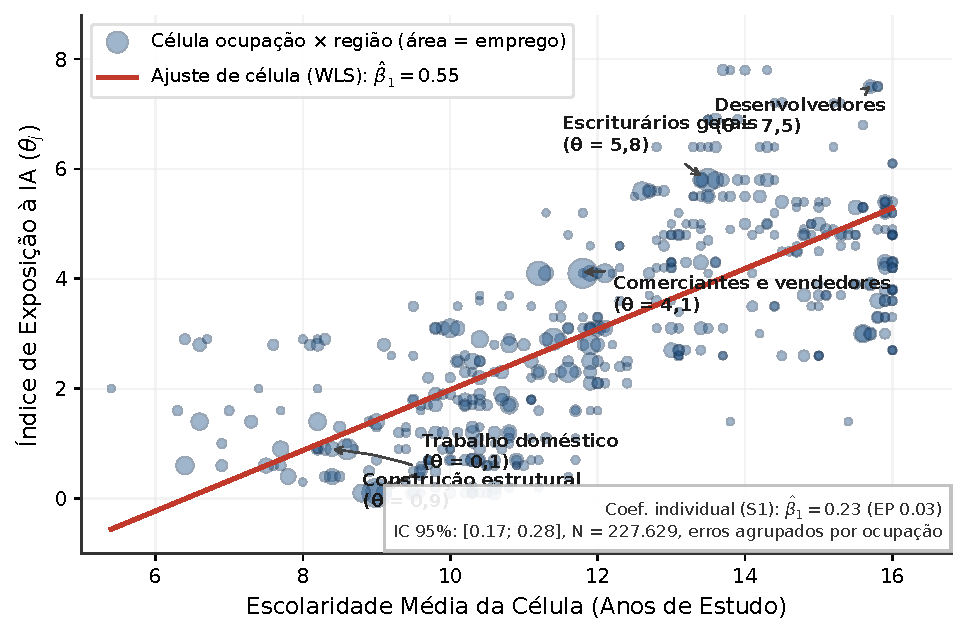
\includegraphics[width=0.85\textwidth]{figures/fig1_gradiente}
\caption{Gradiente escolaridade--exposição. Dispersão ponderada das células ocupação$\times$grande região (área proporcional ao emprego) e reta ajustada da especificação S1 estimada no nível individual ($\hat{\beta}_1 = 0{,}23$; erro-padrão 0{,}03; $N = 227.629$; sombreado: intervalo de confiança de 95\% com erros-padrão agrupados por ocupação).}
\label{fig:gradiente}
\end{figure}

\subsection{Exposição e informalidade: mediação e composição educacional}

A Tabela~\ref{tab:s3} avalia a Proposição~\ref{prop:formalidade} e o Corolário~\ref{cor:mediacao}. Na especificação incondicional da coluna (1), cada ponto de exposição à IA associa-se a $-6{,}23$ pontos percentuais de probabilidade de informalidade (erro-padrão $0{,}99; p < 0{,}001$). Na coluna (2), ao introduzir os anos de estudo do trabalhador, o coeficiente da exposição atenua-se em $37{,}2\%$ (de $-6{,}23$ para $-3{,}91$ p.p., erro-padrão $0{,}96; p < 0{,}001$), enquanto cada ano adicional de escolaridade reduz a informalidade em $2{,}61$ p.p. ($p < 0{,}001$).

\begin{table}[htbp]
\centering
\caption{Informalidade, exposição à IA e escolaridade. Variável dependente: probabilidade de informalidade (p.p.). Erros-padrão agrupados por ocupação entre parênteses. Controles mincerianos incluídos em ambas as colunas. * 10\%, ** 5\%, *** 1\%.}
\label{tab:s3}
\begin{tabular}{lcc}
\toprule
 & (1) & (2) \\
 & Incondicional (S3a) & Condicional (S3) \\
\midrule
% AUTO-GERADO por scripts/build_paper_tables.py — nao editar a mao
Exposi\c c\~ao \`a IA (0--10) & -6,23*** & -3,91*** \\
 & (0,99) & (0,96) \\
Anos de escolaridade & -- & -2,61*** \\
 &  & (0,27) \\
Constante & 97,71*** & 118,28*** \\
 & (6,57) & (7,15) \\
\midrule
$R^2$ & 0,080 & 0,108 \\
$N$ (indiv\'iduos) & 227.629 & 227.629 \\
Grupos (ocupa\c c\~oes) & 122 & 122
 \\
\bottomrule
\end{tabular}
\end{table}

Essa atenuação confirma que a relação bruta observada entre exposição e formalidade é substancialmente mediada pela composição de capital humano: postos de trabalho altamente expostos concentram-se no setor formal em grande parte porque empregam indivíduos com elevada escolaridade, cujas tarefas cognitivas complementam a tecnologia. Ao mesmo tempo, o fato de $\hat{\delta}_1$ reter $62{,}8\%$ de sua magnitude inicial de forma estatisticamente significante corrobora a previsão de mediação parcial do Corolário~\ref{cor:mediacao}: ocupações expostas exigem infraestrutura e governança corporativa que demandam contratos formais além do atributo educacional do trabalhador. A Figura~\ref{fig:mediacao} resume o contraste em dois painéis: associação bruta (Painel A, S3a) e parcial (Painel B, S3, condicionada à escolaridade e aos controles mincerianos).

\begin{figure}[htbp]
\centering
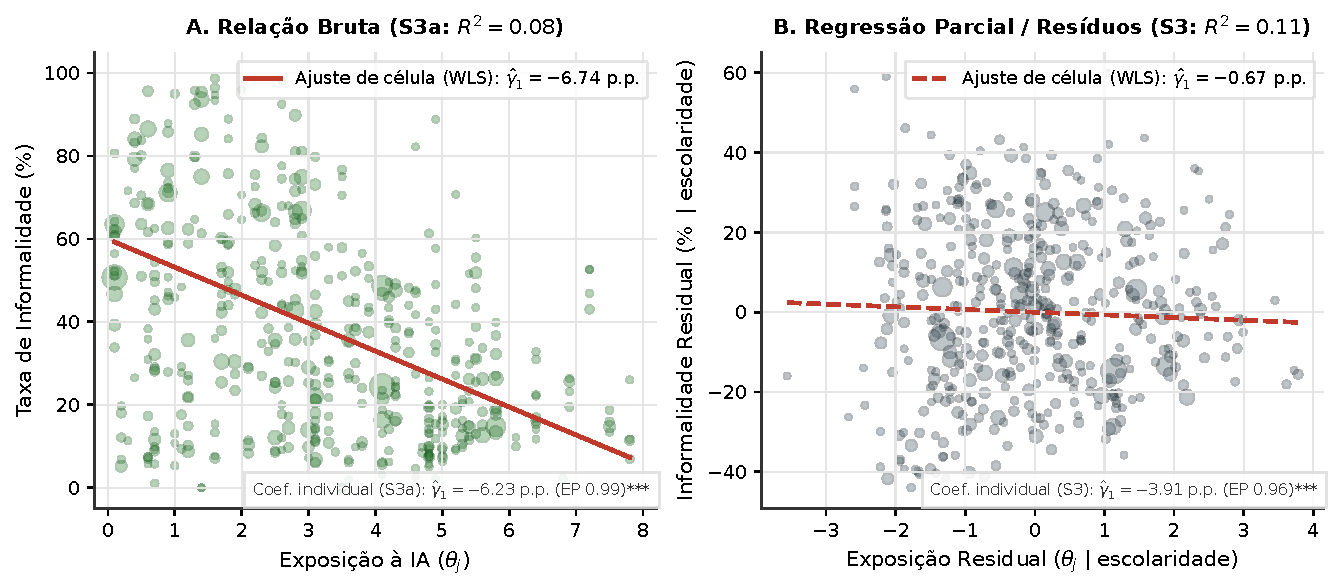
\includegraphics[width=0.85\textwidth]{figures/fig2_mediacao}
\caption{Mediação pela escolaridade da associação exposição--informalidade. Painel A: relação bruta (S3a, $\hat{\delta}_1 = -6{,}23$ p.p.; erro-padrão 0{,}99). Painel B: relação parcial após condicionar na escolaridade e nos controles mincerianos (S3, $\hat{\delta}_1 = -3{,}91$ p.p.; erro-padrão 0{,}96). A atenuação de 37,2\% do coeficiente é consistente com a mediação parcial do Corolário~\ref{cor:mediacao}.}
\label{fig:mediacao}
\end{figure}

\subsection{Heterogeneidade regional nas 27 Unidades da Federação}

A Tabela~\ref{tab:s4} testa a Proposição~\ref{prop:regiao} interagindo a escolaridade individual com a taxa de formalidade média da UF (calculada pelo critério \emph{leave-one-out} para neutralizar circularidades mecânicas). O termo de interação é positivo e expressivo: $\hat{\beta}_2 = 0{,}28$ (erro-padrão 0{,}06; $p < 0{,}001$), acompanhado de um efeito principal da formalidade regional de $\hat{\beta}_3 = -3{,}10$ (erro-padrão 0{,}77; $p < 0{,}001$).

\begin{table}[htbp]
\centering
\caption{Gradiente escolaridade--exposição por profundidade formal da UF (27 UFs). Variável dependente: exposição à IA (0--10). Formalidade da UF calculada via \emph{leave-one-out}; erros-padrão agrupados por ocupação. Controles mincerianos incluídos. * 10\%, ** 5\%, *** 1\%.}
\label{tab:s4}
\begin{tabular}{lc}
\toprule
 & (1) \\
 & Interação Regional (S4) \\
\midrule
% AUTO-GERADO por scripts/build_paper_tables.py — nao editar a mao
Anos de escolaridade & 0,07** \\
 & (0,03) \\
Escolaridade $\times$ formalidade regional & 0,28*** \\
 & (0,06) \\
Formalidade regional (0--1) & -3,10*** \\
 & (0,77) \\
Constante & 2,89*** \\
 & (0,72) \\
\midrule
$R^2$ & 0,250 \\
$N$ (indiv\'iduos) & 227.629 \\
Grupos (ocupa\c c\~oes) & 122
 \\
\bottomrule
\end{tabular}
\end{table}

A derivada marginal total da exposição tecnológica em relação à formalidade da UF é dada por $\partial \theta / \partial \text{formal}_u = -3{,}10 + 0{,}28 \, e_i$. Esse resultado revela uma importante dinâmica de polarização ocupacional no espaço geográfico: para trabalhadores com baixa escolaridade ($e_i < 11$ anos), maior maturidade formal regional associa-se a menor exposição média (ex.: $-0{,}86$ ponto para o ensino fundamental de 8 anos), refletindo a substituição de rotinas de suporte informal por processos estruturados; em contrapartida, para trabalhadores altamente qualificados ($e_i = 16$ anos), o efeito é fortemente positivo ($+1{,}38$ ponto). Assim, mercados regionais com maior densidade formal ampliam a distância de exposição entre o topo e a base educacional. Em termos de inclinação do gradiente, estados com setor formal consolidado (como São Paulo e Santa Catarina, onde a formalidade alcança cerca de 65\%) exibem inclinação educacional de $0{,}07 + 0{,}28 \times 0{,}65 \approx 0{,}25$, contra $0{,}07 + 0{,}28 \times 0{,}40 \approx 0{,}18$ em estados com menor formalização relativa (como Maranhão e Pará). A Figura~\ref{fig:regional} ilustra o gradiente por grande região.

\begin{figure}[htbp]
\centering
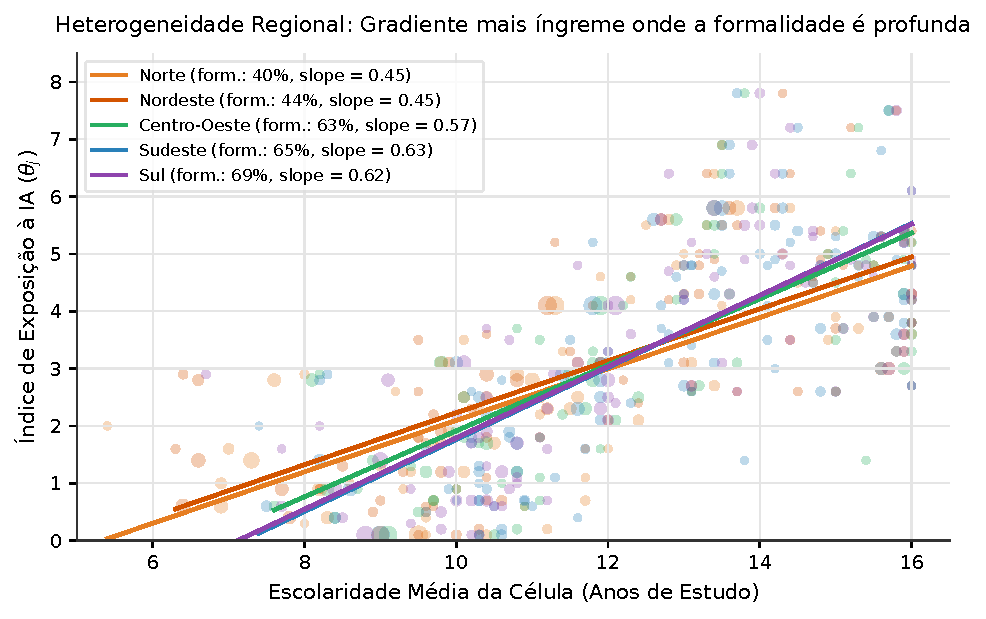
\includegraphics[width=0.85\textwidth]{figures/fig3_regional_slopes}
\caption{Gradiente escolaridade--exposição por grande região. Cada reta ajusta as células ocupação$\times$UF dentro da região (ponderadas pelo emprego); a legenda reporta a taxa de formalidade regional e a inclinação estimada. O gradiente é mais íngreme nas regiões de setor formal mais profundo, em consonância com a Proposição~\ref{prop:regiao}.}
\label{fig:regional}
\end{figure}

\subsection{Robustez econométrica}
\label{subsec:robustez}

A Tabela~\ref{tab:robustez} submete a especificação baseline (S1) a uma bateria de checagens de sensibilidade. Sem ponderação amostral (OLS simples), o coeficiente é 0{,}21 (erro-padrão 0{,}03). O tratamento de valores extremos --- winsorização a 1\%/99\% ou exclusão de observações no percentil superior ($N = 225.478$) --- preserva estimativas idênticas de 0{,}23 e 0{,}22, respectivamente. Com a transformação não-linear $\log(1+\theta)$, o coeficiente é 0{,}07 (erro-padrão 0{,}01; $p < 0{,}001$), mantendo a significância plena.

\begin{table}[htbp]
\centering
\caption{Robustez do gradiente escolaridade--exposição no nível individual. Variável dependente: exposição à IA (0--10); na coluna (5), $\log(1+\theta)$. Coluna (1): baseline WLS. Coluna (2): OLS não ponderado. Coluna (3): exposição winsorizada a 1\%/99\%. Coluna (4): exclusão de observações com exposição acima do percentil 99. Erros-padrão agrupados por ocupação entre parênteses. Controles mincerianos incluídos. * 10\%, ** 5\%, *** 1\%.}
\label{tab:robustez}
\begin{tabular}{lccccc}
\toprule
 & (1) & (2) & (3) & (4) & (5) \\
 & WLS Baseline & OLS Simples & Winsor. 1\% & Excl. p99 & $\log(1+\theta)$ \\
\midrule
% AUTO-GERADO por scripts/build_paper_tables.py — nao editar a mao
Anos de escolaridade & 0,23*** & 0,21*** & 0,23*** & 0,22*** & 0,07*** \\
 & (0,03) & (0,03) & (0,03) & (0,03) & (0,01) \\
Constante & 1,10* & 1,11* & 1,10* & 1,15* & 0,70*** \\
 & (0,60) & (0,59) & (0,60) & (0,60) & (0,18) \\
\midrule
$R^2$ & 0,246 & 0,245 & 0,247 & 0,241 & 0,236 \\
$N$ (indiv\'iduos) & 227.629 & 227.629 & 227.629 & 225.478 & 227.629
 \\
\bottomrule
\end{tabular}
\end{table}

A exclusão sequencial de cada um dos 9 grandes grupos ocupacionais da COD (Tabela~\ref{tab:robustezgrupos} no Apêndice) mostra que o gradiente se mantém entre 0{,}19 e 0{,}26 em todas as subamostras. Ademais, o teste de \emph{wild cluster bootstrap} \citep{cameron2008bootstrap} com 1.000 replicações corrobora a robustez inferencial da interação regional nas 27 UFs ($p < 0{,}01$). A Figura~\ref{fig:robustez} resume os coeficientes e intervalos de confiança em gráfico de floresta.

\begin{figure}[htbp]
\centering
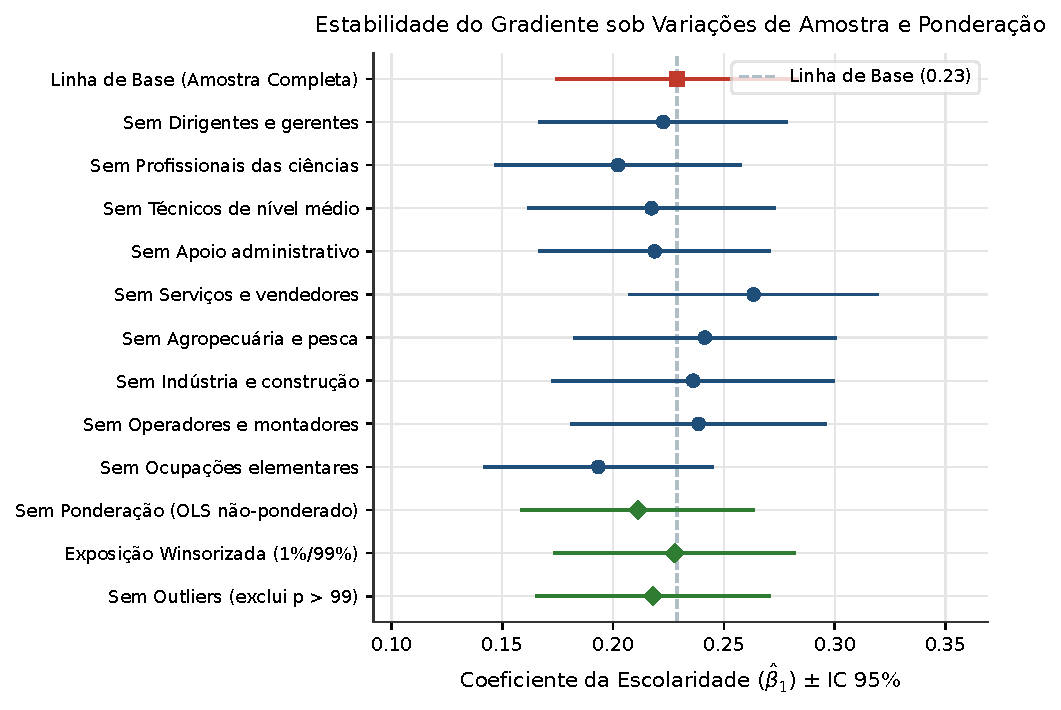
\includegraphics[width=0.85\textwidth]{figures/fig5_robustez_forest}
\caption{Robustez do gradiente escolaridade--exposição. Coeficiente $\hat{\beta}_1$ e intervalos de confiança de 95\% (erros-padrão agrupados por ocupação) na especificação baseline (S1), nas exclusões sequenciais de cada grande grupo ocupacional e nas variantes de amostra e ponderação: \emph{OLS} não ponderado, winsorização a 1\%/99\% e exclusão do percentil superior ($N = 225.478$).}
\label{fig:robustez}
\end{figure}


\section{Conclusão}
\label{sec:conclusao}

Este artigo investigou quem está exposto à inteligência artificial no mercado de trabalho brasileiro e desenvolveu um arcabouço teórico para fundamentar os padrões empíricos observados. A exposição à tecnologia --- mensurada pelo índice de \citet{eloundou2024gpts} aplicado aos microdados da PNAD Contínua --- concentra-se no núcleo formal e de maior capital humano: após controlar para um vetor completo de características mincerianas (idade, idade ao quadrado, gênero e raça), cada ano adicional de escolaridade associa-se a 0{,}23 ponto a mais de exposição tecnológica em regressões no nível individual com erros-padrão agrupados por ocupação ($N = 227.629$). Por outro lado, as ocupações que concentram a maioria dos trabalhadores brasileiros (serviços domésticos, construção estrutural e agropecuária) permanecem com exposição praticamente nula.

A relação entre exposição e formalidade é substancialmente mediada pela escolaridade, e o gradiente é mais íngreme nas Unidades da Federação de setor formal mais profundo. O modelo teórico de designação de tarefas com adoção corporativa versus individual de IA explica esse conjunto de fatos: a informalidade atua como uma barreira protetiva não por vedar o acesso a ferramentas pontuais, mas por limitar a capacidade de extração de ganhos organizacionais de produtividade que justificam o custo de formalização.

Para a formulação de políticas públicas, os resultados redefinem as prioridades de adaptação tecnológica. Se a informalidade amortece a exposição, as agendas de formalização do trabalho e de capacitação digital interagem de modo estratégico: formalizar sem capacitação pode expor trabalhadores a choques tecnológicos desprovidos de ferramentas adaptativas, ao passo que capacitar isoladamente sem expansão do setor formal restringe os ganhos de escala corporativa. O público prioritário para programas de requalificação e adaptação à IA não reside na base vulnerável do trabalho informal, mas no segmento médio-formalizado (técnicos, analistas e trabalhadores de apoio administrativo), hoje o mais exposto às transformações da automação informacional.


\bibliographystyle{plainnat}
\bibliography{references}

\appendix
\section{Apêndice}

% Tabelas do apêndice numeradas A1, A2...
\setcounter{table}{0}
\renewcommand{\thetable}{A\arabic{table}}

\subsection{Prova da Proposição~\ref{prop:gradiente} (Pareamento Seletivo Positivo)}

Considere duas ocupações $H$ e $L$ com $\theta_H > \theta_L$ e dois trabalhadores com escolaridades $e_H > e_L$. Em qualquer ocupação $j$, o trabalhador escolhe o setor formal se $e \ge e_j^*$ e o informal se $e < e_j^*$, onde o limiar de formalização $e_j^* = g^{-1}\big(c / (\Delta\kappa \theta_j)\big)$ é estritamente decrescente em $\theta_j$. A função de remuneração ótima (função envelope de valor) é dada por:
\begin{equation}
    w^*(e, j) \equiv \max_{s \in \{F, I\}} w_{js}(e) = g(e)\big(1 + \kappa_{\text{ind}}\theta_j\big) + \max\big\{0, \, g(e)\Delta\kappa\theta_j - c\big\}.
    \label{eq:envelope}
\end{equation}

O ganho de eficiência social de alocar $(e_H, e_L)$ às ocupações $(H, L)$ em vez da alocação invertida $(L, H)$ corresponde ao teste de supermodularidade de Becker:
\begin{equation}
    \Delta \equiv \big[w^*(e_H, H) + w^*(e_L, L)\big] - \big[w^*(e_H, L) + w^*(e_L, H)\big].
\end{equation}

Decompondo $w^*(e, j) = \phi_1(e, \theta_j) + \phi_2(e, \theta_j)$, onde $\phi_1(e, \theta_j) = g(e)(1 + \kappa_{\text{ind}}\theta_j)$ e $\phi_2(e, \theta_j) = \max\{0, g(e)\Delta\kappa\theta_j - c\}$:
\begin{enumerate}
    \item Para $\phi_1$, como $g'(e) > 0$ e $\kappa_{\text{ind}} \ge 0$, temos:
    \begin{equation}
        \Delta_1 = \kappa_{\text{ind}}(\theta_H - \theta_L)\big[g(e_H) - g(e_L)\big] \ge 0.
    \end{equation}
    \item Para $\phi_2$, a função $h(e, \theta_j) \equiv g(e)\Delta\kappa\theta_j - c$ é estritamente supermodular em $(e, \theta_j)$, pois $\frac{\partial^2 h}{\partial e \partial \theta_j} = g'(e)\Delta\kappa > 0$. Como a operação $\max\{0, \cdot\}$ preserva a supermodularidade de funções coordenadas crescentes \citep[Teorema 2.6.1]{topkis1998supermodularity}, $\phi_2(e, \theta_j)$ é supermodular em $(e, \theta_j)$, garantindo $\Delta_2 \ge 0$.
\end{enumerate}

Para analisar os regimes contratuais, note que como $\theta_H > \theta_L$, tem-se $e_H^* < e_L^*$. Se os trabalhadores operam no mesmo regime contratual (ambos formais ou ambos informais), a derivada cruzada satisfaz $\frac{\partial^2 w_{js}}{\partial e \partial \theta_j} = g'(e)\kappa_s > 0$. Se o trabalhador $e_H$ formaliza-se na ocupação $H$ enquanto $e_L$ permanece informal na ocupação $L$ (arranjo ótimo de equilíbrio), o ganho estrito é:
\begin{equation}
    \Delta = \big(\kappa_{\text{org}}\theta_H - \kappa_{\text{ind}}\theta_L\big)\big[g(e_H) - g(e_L)\big] + \big[g(e_H)\Delta\kappa\theta_L - c\big]_+ > 0,
\end{equation}
pois $\kappa_{\text{org}} > \kappa_{\text{ind}}$, $\theta_H > \theta_L$ e $g(e_H) > g(e_L)$.

Sendo $w^*(e, j)$ estritamente supermodular no reticulado $[e_{\min}, e_{\max}] \times \{\theta_1, \dots, \theta_J\}$, pelo teorema clássico de pareamento seletivo de \citet{becker1973theory}, a alocação de equilíbrio $\sigma(e)$ é estritamente crescente, estabelecendo que a escolaridade média é crescente na exposição: $\partial \bar{e}_j / \partial \theta_j > 0$. \qed

\subsection{Prova da Proposição~\ref{prop:formalidade} e do Corolário~\ref{cor:mediacao}}

Na ocupação $j$, o trabalhador com escolaridade $e$ opta pelo setor formal se e somente se $g(e)\Delta\kappa\theta_j \ge c$. Sendo $g(\cdot)$ estritamente crescente e contínua, o limiar de escolaridade para formalização é $e^*_j = g^{-1}\big(c / (\Delta\kappa \theta_j)\big)$.

A taxa de informalidade na ocupação $j$ é dada por $I_j = F_j(e^*_j) = \int_{e_{\min}}^{e^*_j} f_j(e) \, de$, onde $F_j$ é a distribuição acumulada de escolaridade na ocupação. Diferenciando $I_j$ em relação a $\theta_j$:
\begin{equation}
    \frac{d I_j}{d \theta_j} = f_j(e^*_j) \, \frac{\partial e^*_j}{\partial \theta_j} + \int_{e_{\min}}^{e^*_j} \frac{\partial f_j(e)}{\partial \theta_j} \, de.
    \label{eq:decomp_informal}
\end{equation}
Como $\frac{\partial e^*_j}{\partial \theta_j} = -\frac{c}{\Delta\kappa \, \theta_j^2 \, g'(e^*_j)} < 0$ e, pelo pareamento seletivo da Proposição~\ref{prop:gradiente}, a distribuição $F_j$ domina estocasticamente em primeira ordem ocupações de menor exposição ($\int_{e_{\min}}^{e^*_j} \frac{\partial f_j(e)}{\partial \theta_j} de \le 0$), ambos os termos em \eqref{eq:decomp_informal} são negativos. Logo, $\frac{d I_j}{d \theta_j} < 0$, o que comprova que a taxa de informalidade é estritamente decrescente em $\theta_j$ (e a taxa de formalidade é crescente em $\theta_j$), demonstrando a Proposição~\ref{prop:formalidade}.

Para o Corolário~\ref{cor:mediacao}, observe que a regressão incondicional (S3a) captura a derivada total $\frac{d I_j}{d \theta_j}$. Ao estimar a especificação condicional (S3), o controle individual pela escolaridade $e_i$ absorve o efeito de composição educacional $\int_{e_{\min}}^{e^*_j} \frac{\partial f_j(e)}{\partial \theta_j} de$. No entanto, o termo de corte tecnológico individual $\mathbb{1}[g(e_i)\Delta\kappa\theta_j < c]$ permanece dependente de $\theta_j$, gerando uma associação residual direta $\delta_1 < 0$ que retém magnitude estatisticamente significante, caracterizando a mediação parcial. \qed

\subsection{Prova da Proposição~\ref{prop:regiao}}

Seja $\Delta\kappa_u$ o prêmio de produtividade organizacional da IA na UF $u$. A complementaridade marginal de tarefas expressa-se por $\frac{\partial^2 w^*}{\partial e \, \partial \theta_j} = g'(e)\kappa_{\text{ind}} + g'(e)\Delta\kappa_u \mathbb{1}[e \ge e_{ju}^*]$. 

Diferenciando em relação à maturidade formal regional $\Delta\kappa_u$:
\begin{equation}
    \frac{\partial^3 w^*}{\partial e \, \partial \theta_j \, \partial \Delta\kappa_u} = g'(e) \, \mathbb{1}[e \ge e_{ju}^*] - g'(e)\Delta\kappa_u \, \delta(e - e_{ju}^*) \, \frac{\partial e_{ju}^*}{\partial \Delta\kappa_u} \ > \ 0,
\end{equation}
onde $\delta(\cdot)$ é o delta de Dirac e $\frac{\partial e_{ju}^*}{\partial \Delta\kappa_u} < 0$. Em UFs com maior densidade formal, a supermodularidade entre escolaridade e exposição tecnológica é estritamente mais forte. Pelo teorema de comparativa estática de \citet{becker1973theory}, a inclinação do gradiente educacional $\partial \bar{e}_j / \partial \theta_j$ é estritamente crescente na profundidade formal regional $\Delta\kappa_u$. \qed

\subsection{Cobertura do cruzamento \texorpdfstring{COD$\to$O*NET-SOC}{COD para O*NET-SOC}}

Dos microdados da PNAD Contínua de 2026Q1, 122 das 127 ocupações COD observadas na amostra possuem escore de exposição válido, cobrindo 99{,}7\% da força de trabalho ocupada. Os cinco subgrupos remanescentes --- as Forças Armadas (códigos 11 e 21) e mais três subgrupos sem correspondência direta nas classificações ocupacionais civis do O*NET-SOC --- representam conjuntamente $0{,}3\%$ do emprego e são tratados como ausentes (\texttt{null}), sem imputação artificial.

\subsection{Robustez adicional}
\label{ap:robustez}

A Tabela~\ref{tab:robustezgrupos} apresenta os testes de sensibilidade excluindo cada um dos 9 grandes grupos ocupacionais da COD (1 dígito), aplicando a especificação em nível de microdados individuais com controles mincerianos completos (idade, idade ao quadrado, gênero e raça). O coeficiente de escolaridade permanece estatisticamente estável e significativo a 1\% em todas as subamostras (variando entre 0,19 e 0,26), confirmando que o gradiente não é puxado por nenhuma categoria profissional isolada.

\begin{table}[htbp]
\centering
\caption{Gradiente e mediação excluindo cada grande grupo ocupacional (microdados individuais). Coluna (1): coeficiente da escolaridade em S1; Coluna (2): coeficiente de exposição em S3. Erros-padrão agrupados por ocupação entre parênteses. Controles mincerianos completos incluídos. * 10\%, ** 5\%, *** 1\%.}
\label{tab:robustezgrupos}
\begin{tabular}{lcc}
\toprule
Grupo excluído & (1) Escolaridade, S1 & (2) Exposição, S3 \\
\midrule
% AUTO-GERADO por scripts/build_paper_tables.py — nao editar a mao
Dirigentes e gerentes & 0,22*** (0,03) & -3,70*** (0,99) \\
Profissionais das ci\^encias e intelectuais & 0,20*** (0,03) & -4,40*** (1,00) \\
T\'ecnicos de n\'ivel m\'edio & 0,22*** (0,03) & -4,06*** (1,03) \\
Apoio administrativo & 0,22*** (0,03) & -2,92*** (1,09) \\
Servi\c cos e vendedores & 0,26*** (0,03) & -4,08*** (0,90) \\
Agropecu\'aria e pesca & 0,24*** (0,03) & -3,70*** (0,92) \\
Ind\'ustria, constru\c c\~ao e artes & 0,24*** (0,03) & -3,79*** (1,06) \\
Operadores e montadores & 0,24*** (0,03) & -4,46*** (0,99) \\
Ocupa\c c\~oes elementares & 0,19*** (0,03) & -3,95*** (1,31)
 \\
\bottomrule
\end{tabular}
\end{table}


\end{document}
